\chapter{Plugins}\label{sec:plugins}

Most of the plugins described ib this chapter are also in the Wiki. Texts and figures have been copied from the Wiki but adapted to be included in Latex documents (Miktex 2.9).

\section{General}

\codeblocks' features can be extend by using plugins. There are generally three types of plugins:
\begin{description}
\item[Core plugins:] developed and maintained by the core C::B team.
\item[Contrib plugins:] developed and maintained by the community and proven to be very valuable. So they are integrated into the C::B SVN.
\item[3rd party plugins:] developed and maintained by the community but not (yet?) in the C::B repository. Theses plugins often have their own repository or are being posted (including the source code) in the forums.
\end{description}

\textbf{If you are looking for plugins}:
\begin{enumerate}
\item Look in the official release. Notice that the installer / package manager might require you to enable some of the plugins specifically. So READ carefully.
\item Search the forums for announcements, especially the forums at \url{http://forums.codeblocks.org/index.php/board,14.0.html}.
\item There might be information on the Wiki concerning other plugins on this page and here : \url{http://Wiki.codeblocks.org/index.php/Announcement_for_plugins/patches}.
\end{enumerate}

For Windows users, the default behavior of the current installer does \textbf{not} install contrib plugins. You need to manually check the "contrib plugin" checkbox when asked for selected components to install. There is no way to install them manually afterwards.


\textbf{If you are developing plugins}: Surely you can work with plugin as you like, but here are some suggestions:

\tab Announce them in the plugin development board in the forums - including the (initial) source code.

OR

\tab Setup your own webpage (or use a file sharing platform) and post the link to the sources/binaries/svn access in the plugin development board in the forums.

OR

\tab Setup a repository, probably at BerliOS or SourceForge, post the link to the sources/binaries/svn access in the plugin development board in the forums. Notice: This is very convenient as attachments in our forum might be deleted from time to time. So it is not safe to post source code in the forums.

THEN

\tab Enter the plugins description on this page.

\tab Announce the plugin using this template on \url{http://Wiki.codeblocks.org/index.php/Template_for_plugin_announcement}

\begin{ASTYLE}
\section{Astyle}\label{sec:astyle}

Artistic Style is a source code indenter, source code formatter, and source code beautifier for the C, C++, C\# programming languages. It can be used to select different styles of coding rules within \codeblocks.

\screenshot{astyle}{Formating your source code}

When indenting source code, we as programmers have a tendency to use both spaces and tab characters to create the wanted indentation. Moreover, some editors by default insert spaces instead of tabs when pressing the tab key, and other editors have the ability to prettify lines by automatically setting up the white space before the code on the line, possibly inserting spaces in a code that up to now used only tabs for indentation.

Since the number of space characters shown on screen for each tab character in the source code changes between editors, one of the standard problems programmers are facing when moving from one editor to another is that code containing both spaces and tabs that was up to now perfectly indented, suddenly becomes a mess to look at when changing to another editor. Even if you as a programmer take care to ONLY use spaces or tabs, looking at other people's source code can still be problematic.

To address this problem, Artistic Style was created - a filter written in C++ that automatically re-indents and re-formats C / C++ / C\# source files.

\hint{When copying code, for example from the internet or a manual, this code will automatically be adapted to the coding rules in \codeblocks.}

\end{ASTYLE}

\begin{AUTOVERSIONING}
\section{AutoVersioning}\label{sec:autoversioning}

An application versioning plug in that increments the version and build number of your application every time a change has been made and stores it in \file{version.h} with easy to use variable declarations. Also have a feature for committing changes a la SVN style, a version scheme editor, a change log generator and more $\ldots$

\subsection{Introduction}

The idea of the AutoVersioning plugin was made during the development of a pre-alpha software that required the version info and status. Been to busy coding, without time to maintain the version number, just decided to develop a plugin that could do the job with little intervention as possible.

\subsection{Features}

Here is the list of features the plugin covers summarized:

\begin{itemize}
\item Supports C and C++.
\item Generates and auto increment version variables.
\item Software status editor.
\item Integrated scheme editor for changing the behavior of the auto incrementation of version values.
\item Date declarations as month, date and year.
\item Ubuntu style version.
\item Svn revision check.
\item Change log generator.
\item Works on Windows and Linux.
\end{itemize}

\subsection{Usage}

Just go to \menu{Project,Autoversioning} menu. A pop up window like this will appear:

\figures[H][width=.45\columnwidth]{autoversion_configure}{Configure project for Autoversioning}

When hitting yes on the ask to configure message box, the main auto versioning configuration dialog will open, to let you configure the version info of your project.

After configuring your project for auto versioning, the settings that you entered on the configuration dialog will be stored on the project file, and a \file{version.h} file will be created. For now, every time that you hit the \menu{Project,Autoversioning} menu the configuration dialog will popup to let you edit your project version and versioning related settings, unless you don't save the new changes made by the plugin to the project file.

\subsection{Dialog notebook tabs}
\genterm{Version Values}

Here you just enter the corresponding version values or let the auto versioning plugin increment them for you (see \pxref{fig:autoversion_editor}).

\begin{description}
\item[Major] Increments by 1 when the minor version reaches its maximum
\item[Minor] Increments by 1 when the build number pass the barrier of build times, the value is reset to 0 when it reach its maximum value.
\item[Build Number] (also equivalent to Release) - Increments by 1 every time that the revision number is incremented.
\item[Revision] Increments randomly when the project has been modified and then compiled.
\end{description}

\screenshot{autoversion_editor}{Set Version Values}

\genterm{Status}

Some fields to keep track of your software status with a list of predefined values for convenience(see \pxref{fig:autoversion_status}).

\begin{description}
\item[Software Status] The typical example should be v1.0 Alpha
\item[Abbreviation] Same as software status but like this: v1.0a
\end{description}

\screenshot{autoversion_status}{Set Status of Autoversioning}

\genterm{Scheme}

Lets you edit how the plugin will increment the version values (see \pxref{fig:autoversion_scheme}).

\screenshot{autoversion_scheme}{Scheme of autoversioning}

\begin{description}
\item[Minor maximum] The maximum number that the Minor value can reach, after this value is reached the Major is incremented by 1 and next time project is compiled the Minor is set to 0.
\item[Build Number maximum] When the value is reached, the next time the project is compiled is set to 0. Put a 0 for unlimited.
\item[Revision maximum] Same as Build Number maximum. Put a 0 for unlimited
\item[Revision random maximum] The revision increments by random numbers that you decide, if you put here 1, the revision obviously will increment by 1.
\item[Build times before incrementing Minor] After successful changes to code and compilation the build history will increment, and when it reaches this value the Minor will increment.
\end{description}

\genterm{Settings}

Here you can set some settings of the auto versioning behavior (see \pxref{fig:autoversion_settings}).

\screenshot{autoversion_settings}{Settings of Autoversioning}

\begin{description}
\item[Autoincrement Major and Minor] Lets the plugin increments this values by you using the scheme. If not marked only the Build Number and Revision will increment.
\item[Create date declarations] Create entries in the \file{version.h} file with dates and ubuntu style version.
\item[Do Auto Increment] This tells the plugin to automatically increment the changes when a modification is made, this incrementation will occur before compilation.
\item[Header language] Select the language output of \file{version.h}
\item[Ask to increment] If marked, Do Auto Increment, it ask you before compilation (if changes has been made) to increment the version values.
\item[svn enabled] Search for the svn revision and date in the current folder and generates the correct entries in \file{version.h}
\end{description}

\genterm{Changes Log}

This lets you enter every change made to the project to generate a \file{ChangesLog.txt} file (see \pxref{fig:autoversion_changelog}).

\screenshot{autoversion_changelog}{Changelog of Autoversioning}

\begin{description}
\item[Show changes editor when incrementing version] Will pop up the changes log editor when incrementing the version.
\item[Title Format] A format able title with a list of predefined values.
\end{description}

\subsection{Including in your code}

To use the variables generated by the plugin just \codeline{\#include <version.h>}. An example code would be like the following:

\begin{lstlisting}
#include <iostream>
#include "version.h"

void main(){
    std::cout<<AutoVersion::Major<<endl;
}
\end{lstlisting}

\genterm{Output of version.h}

The generated header file. Here is a sample content of the file on c++ mode:

\begin{lstlisting}
#ifndef VERSION_H
#define VERSION_H

namespace AutoVersion{

	//Date Version Types
	static const char DATE[] = "15";
	static const char MONTH[] = "09";
	static const char YEAR[] = "2007";
	static const double UBUNTU_VERSION_STYLE = 7.09;

	//Software Status
	static const char STATUS[] = "Pre-alpha";
	static const char STATUS_SHORT[] = "pa";

	//Standard Version Type
	static const long MAJOR = 0;
	static const long MINOR = 10;
	static const long BUILD = 1086;
	static const long REVISION = 6349;

	//Miscellaneous Version Types
	static const long BUILDS_COUNT = 1984;
	#define RC_FILEVERSION 0,10,1086,6349
	#define RC_FILEVERSION_STRING "0, 10, 1086, 6349\0"
	static const char FULLVERSION_STRING[] = "0.10.1086.6349";

}
#endif //VERSION_h
\end{lstlisting}

On C mode is the same as C++ but without the namespace:

\begin{lstlisting}
#ifndef VERSION_H
#define VERSION_H

	//Date Version Types
	static const char DATE[] = "15";
	static const char MONTH[] = "09";
	static const char YEAR[] = "2007";
	static const double UBUNTU_VERSION_STYLE = 7.09;

	//Software Status
	static const char STATUS[] = "Pre-alpha";
	static const char STATUS_SHORT[] = "pa";

	//Standard Version Type
	static const long MAJOR = 0;
	static const long MINOR = 10;
	static const long BUILD = 1086;
	static const long REVISION = 6349;

	//Miscellaneous Version Types
	static const long BUILDS_COUNT = 1984;
	#define RC_FILEVERSION 0,10,1086,6349
	#define RC_FILEVERSION_STRING "0, 10, 1086, 6349\0"
	static const char FULLVERSION_STRING[] = "0.10.1086.6349";

#endif //VERSION_h
\end{lstlisting}

\subsection{Change log generator}

This dialog is accessible from the menu \menu{Project,Changes Log}. Also if checked Show changes editor when incrementing version on the changes log settings, the window will open to let you enter the list of changes after a modification to the project sources or an incrementation event (see \pxref{fig:autoversion_changes}).

\screenshot{autoversion_changes}{Changes for a project}

\genterm{Buttons Summary}

\begin{description}
\item[Add] Appends a row in to the data grid
\item[Edit] Enables the modification of the selected cell
\item[Delete] Removes the current row from the data grid
\item[Save] Stores into a temporary file (\file{changes.tmp}) the actual data for later processing into the changes log file
\item[Write] Process the data grid data to the changes log file
\item[Cancel] Just closes the dialog without taking any action
\end{description}

Here is an example of the output generated by the plugin to the \file{ChangesLog.txt} file:

\begin{code}
03 September 2007
   released version 0.7.34 of AutoVersioning-Linux

     Change log:
        -Fixed: pointer declaration
        -Bug: blah blah

02 September 2007
   released version 0.7.32 of AutoVersioning-Linux

     Change log:
        -Documented some areas of the code
        -Reorganized the code for readability

01 September 2007
   released version 0.7.30 of AutoVersioning-Linux

     Change log:
        -Edited the change log window
        -If the change log windows is leave blank no changes.txt is modified
\end{code}

\end{AUTOVERSIONING}

\begin{BROWSETRACKS}
\section{BrowseTracks}\label{sec:browsetracks}

BrowseTracker is a plugin that helps navigating between recently opened files in \codeblocks. The list of recent files is saved in a history. The number of entries is limited to 20. With the menu \menu{View,Browse Tracker,Clear} the history is cleared.

With the window \samp{Browsed Tabs} you can navigate between the items of the recently opened files using the menu entry \menu{View,Browse Tacker,forward/backward} or the shortcut Alt-Left/Alt-Right.

A common procedure when developing software is to struggle with a set of functions which are implemented in different files. The BrowseTracks plugin will help you solve this problem by showing you the order in which the files were selected. You can then comfortably navigate the function calls.

The configuration of the plugin is stored in your application data directory in the file \file{default.conf}. If you use the personality feature of \codeblocks the configuration is read from the file \file{\var{personality}.conf}.


\end{BROWSETRACKS}

\begin{CODESNIPPETS}
\section{CodeSnippets}\label{sec:codesnippets}

The CodeSnippets plug-in makes it possible to structure text modules and links to files according to categories in a tree view. The modules are used for storing often used files and constructs in text modules and managing them in a central place. Imagine the following situation: A number of frequently used source files are stored in different directories of the file system. The CodeSnippets window provides the opportunity to create categories, and below the categories, links to the required files. With these features, you can control the access to the files independently from where they are stored within the file system, and you can navigate quickly between the files without the need to search the whole system.

\hint{You can use \codeblocks variables or environment variables in file links e.g. \codeline{$(VARNAME)/name.pdf} to parametrise a link in the CodeSnippets browser.}

The list of text modules and links can be stored in the CodeSnippets window by right-clicking and selecting \samp{Save Index} from the context menu. The file \file{codesnippets.xml} which will be created by this procedure, can then be found in the \file{codeblocks} subdirectory of your \file{Documents and Settings\osp Application data} directory. Under Linux, this information is stored in the \file{.codeblocks} subdirectory of your HOME directory. The \codeblocks configuration files will be loaded during the next start-up. If you wish to save the content of CodeSnippets at a different location, select the \samp{Save Index As} entry. To load this file, select \samp{Load Index File} during the next start-up of \codeblocks or include the directory in the \samp{Settings} context menu under \samp{Snippet Folder}. The settings are saved in the corresponding file \file{codesnippets.ini} in your application data.

For including a category, use the \samp{Add SubCategory} menu. A category can contain Snippets (text modules) or File Links. A text module is created via the \samp{Add Snippet} command in the context menu. The content is integrated into the text module as \samp{New snippet} by selecting the text passage in the \codeblocks editor and dragging and dropping it onto the module and the properties dialog pops up. Double-clicking the newly included entry or selecting \samp{Edit Text} will open an editor for the content.

\screenshot{edit_snippet}{Editing a text module}

Output of a text module is handled in \codeblocks via the context menu command \samp{Apply} or by dragging and dropping into the editor. Under Windows, the contents of a Snippet can also be dragged and dropped into other applications. In the CodeSnippets Browser you can copy a selected item with drag and drop to a different category.

Beyond this, text modules can be parametrised by \var{name} variables which can be accessed via \codeline{$(name)} (see \pxref{fig:edit_snippet}). The values of the variables can be retrieved in an entry field if the text module is called via the context menu command \samp{Apply}.

Besides the text modules, links to files can also be created. If, after having created a text module, you click the context menu command \samp{Properties}, then you can select the link target by clicking the \samp{Link target} button. This procedure will automatically convert the text module into a link to a file. In CodeSnippets, all text modules will be marked by a T symbol, links to a file by an F symbol and urls by an U symbol. If you want to open a selected file (link) in the codesnippets view just select the context menu \menu{Open File} or hold the \samp{Alt} key and make a double click on the file.

\hint{You can add even url (e.g. http://www.codeblocks.org) in text modules. The url will be opened in your favorite browser with the context menu \menu{Open Url}.}
%\hint{If you have chosen the setting \samp{open it with the associated application} under \menu{Settings,Environment} for file extension handling, the application assigned by Windows for the file extension will be used (see \pxref{sec:file_extension}).}

With this setting, if open a link to a pdf file from the codesnippets view a pdf viewer will be started automatically. This method makes it possible for a user to access files which are spread over the whole network, such as cad data, layouts, documentations etc., with the common applications, simply via the link. The content of the codesnippets is stored in the file \file{codesnippets.xml}, the configuration is stored in the file \file{codesnippets.ini} in your \file{application data} directory. This ini file will, for example, contain the path of the file \file{codesnippets.xml}.

\codeblocks supports the usage of different profiles. These profiles are called personalities. Starting \codeblocks with the command line option \opt{--personality=\var{profile}} will create a new or use an existing profile. Then the settings will not be stored in the file \file{default.conf}, but in \file{\var{personality}.conf} in your \file{application data} directory instead. The Codesnippets plugin will then store its settings in the file \file{\var{personality}.codesnippets.ini}. Now, if you load a new content \file{\var{name.xml}} in the Codesnippets settings via \samp{Load Index File}, this content will be stored in the corresponding ini file. The advantage of this method lies in the fact that in case of different profiles, different configurations for text modules and links can be managed.

The plug-in offers an additional search function for navigating between the categories and Snippets. The scope for searching Snippets, categories or Snippets and categories can be adjusted. By entering the required search expression, the corresponding entry is automatically selected in the view. \pxref{fig:codesnippets} shows a typical display in the CodeSnippets window.

\figures[hbt!][width=.4\columnwidth]{codesnippets}{CodeSnippets View}

\hint{When using voluminous text modules, the content of these modules should be saved in files via \samp{Convert to File Link} in order to reduce memory usage within the system. If you delete a codesnippet or file link it will be moved to the category \file{.trash}; if you hold the Shift key the item will be deleted.}

\end{CODESNIPPETS}

\begin{DOXYBLOCKS}
\section{Doxyblocks}\label{sec:doxyblocks}

DoxyBlocks is a plugin for \codeblocks that integrates doxygen into the IDE. It allows you to create documentation, insert comment blocks and run HTML or CHM documents. It also provides configuration of some of the more commonly used settings and access to doxywizard for more detailed configuration.

The settings in the DoxyBlocks toolbar have the following meanings:

\begin{description}
\item[
\includegraphics{Doxywizard}] Run doxywizard. Ctrl-Alt-D
\item[
\includegraphics{Extract}] Extract documentation for the current project. Ctrl-Alt-E
\item[
\includegraphics{Comment_block}] Insert a comment block at the current line. Additionally, DoxyBlocks will try to intelligently read if a method exists on the line for which a comment is being added. Ctrl-Alt-B

\begin{lstlisting}
/** \brief
 *
 * \param bar bool
 * \return void
 *
 */    
void MyClass::Foo(bool bar)
{
    fooBar(bar);
}
\end{lstlisting}

\item[
\includegraphics{Comment_line}] Insert a line comment at the current cursor position. Ctrl-Alt-L
\begin{lstlisting}
void MyClass::Foo(bool bar)
{
    fooBar(bar); /**<  */
}
\end{lstlisting}

\item[
\includegraphics{Html}] View generated HTML documentation. Ctrl-Alt-H
\item[
\includegraphics{Chm}] View generated HTML Help documentation. Ctrl-Alt-C
\item[
\includegraphics{Configure}] Open DoxyBlocks' preferences. Ctrl-Alt-P
\end{description}

Doxyblocks works only if doxygen is installed on your system. You need at least the executables doxygen and doxywizard (available in official doxygen distribution at \url{http://www.doxygen.nl/}). Optionally you can have the executable "dot" from the graphviz package (see \url{https://graphviz.gitlab.io/}. On Windows, the help compiler (hhc) may be used to generate chm files.

\genterm{Notes}
\begin{description}
\item In the preferences you have a check box to allow or not allow DoxyBlocks to \textbf{overwrite the doxyfile}. By default, if a doxyfile already exists it is not overwritten to protect any changes that have been made outside DoxyBlocks however this behaviour prevents changes made within DoxyBlocks being written to an existing doxyfile.
\item If a text field is blank in "Preferences", DoxyBlocks will assume that the corresponding executable is available somewhere in your environment's path. You can use macros such as \$(CODEBLOCKS) in your path and they will be expanded automatically.
\item [OUTPUT\_DIRECTORY] Used to specify the (relative or absolute) base path where the generated documentation will be put. If a relative path is entered, it will be relative to the location where doxygen was started. If left blank the current directory will be used. DoxyBlocks will use the path name entered here to create a directory relative to \codeline{<project dir>}. This allows you to create separate doxygen directories for projects that reside in the same directory, or just use a different directory name. If this field is blank, documents will be created in \codeline{<project dir>/doxygen}. Enter directory names without dots, leading separators, volume names, etc. DoxyBlocks does validation on the path name and will strip extraneous characters.
\begin{lstlisting}
Examples:
[blank]           -> <project dir>/doxygen.
"docs"            -> <project dir>/docs.
"docs/sub1/sub2"  -> <project dir>/docs/sub1/sub2.
"doxygen/docs"    -> <project dir>/doxygen/docs.
\end{lstlisting}
\item [OUTPUT\_LANGUAGE] Used to specify the language in which all documentation generated by doxygen is written. Doxygen will use this information to generate all constant output in the proper language. The default language is English. Other languages are supported. 
\item More information in doxygen help files
\end{description}
\end{DOXYBLOCKS}

\begin{EDITORTWEAKS}
\section{Editor Tweaks plugin}\label{sec:editor_tweaks}

The EditorTweaks plugin contains several different features. On a per-file basis, it controls :

\begin{itemize}
\item word-wrap;
\item line-numbers;
\item tab key emissions (tab characters or spaces);
\item number of spaces the tab key emits;
\item end of line characters (carriage-return + linefeed; carriage-return; linefeed);
\item visibility of end of line characters;
\item on-demand striping of trailing white-space;
\item on-demand synchronization of end of line characters;
\item insert key suppression.
\end{itemize}

From the merge with the Aligner plugin, it has the ability to make sections of code more readable by aligning a specific character. For example, aligning the "=" in 

\begin{lstlisting}
int var = 1;
int longVarName = 2;
int foobar = 3;
\end{lstlisting}

will result in:

\begin{lstlisting}
int var         = 1;
int longVarName = 2;
int foobar      = 3;
\end{lstlisting}



\end{EDITORTWEAKS}

\begin{FILEMANAGER}
\section{File Explorer and Shell Extension Plugin}\label{sec:file_explorer}

The File Explorer \pxref{fig:file_explorer} is included in the Shell Extensions plugin, and can be found in the \samp{Files} tab. The composition of the File Explorer is shown in \pxref{fig:file_explorer}.

On top you will find a field for entering the path. By clicking the button at the end of this field, the drop-down field will list a history of the past entries which can be navigated via a scroll bar. The up arrow key on the right-hand side of the field moves up the directory structure one directory.

In the \samp{Wildcard} field you can enter a filter term for the file display. Leaving the field empty or entering \codeline{*} results in all files being displayed. Entering \codeline{*.c;*.h}, for example will result in solely C sources and header files being displayed. Opneing the pull-down field will, again, list a history of the last entries.

\figures[hbt!]{file_explorer}{The file manager}

Pressing the Shift key and clicking selects a group of files or directories, pressing the Ctrl key and clicking selects multiple separate files or directories.

The following operations can be started via the context menu if one or multiple directories are selected in the File Explorer:

\begin{description}
\item[Make Root] defines the current directory as the root directory.
\item[Add to Favorites] sets a marker for the directory and stores it as a favourite. This function allows you to navigate quickly between frequently used directories, also on different network drives.
\item[New File] creates a new file in the selected directory.
\item[Make Directory] creates a new subdirectory in the selected directory.
\end{description}

The following operations can be started via the context menu if one or multiple files or directories are selected in the File Explorer:

\begin{description}
\item[Duplicate] copies a file/directory and renames it.
\item[Copy To] opens a dialogue for entering the target directory in which the copied file/directory is to be stored.
\item[Move To] moves the selection to the target location.
\item[Delete] deletes the selected files/directories.
\item[Show Hidden Files] activates/deactivates the display of hidden system files. When activated, this menu entry is checkmarked.
\item[Refresh] update the display of the directory tree.
\end{description}

The following operations can be started via the context menu if one or multiple files are selected in the File Explorer:

\begin{description}
\item[Open in CB Editor] opens the selected file in the \codeblocks editor.
\item[Rename] renames the selected file.
\item[Add to active project] adds the file(s) to the active project.
\end{description}

\hint{The files/directories selected in the File Explorer can be accessed in the Shell Extensions plugin via the \codeline{mpaths} variable.}

User-defined functions can be specified via the menu command \menu{Settings,Environment,Shell Extensions}. In the Shell Extensions mask, a new function which can be named at random, is created via the \samp{New} button. In the \samp{ShellCommand Executable} field, the executable program is stated, and in the field at the bottom of the window, additional parameters can be passed to the program.
By clicking the function in the context menu or the Shell Extensions menu, the function is started and will then process the selected files/directories. The output is redirected to a separate shell window.

For example a menu entry in \menu{Shell Extensions,SVN} and in the context menu is created for \samp{SVN}. \codeline{$file} in this context means the file selected in the File Explorer, \codeline{$mpath} the selected files or directories (see \pxref{sec:builtin_variables}).

\begin{code}
 Add;$interpreter add $mpaths;;;
\end{code}

This and every subsequent command will create a submenu, in this case called \menu{Extensions,SVN,Add}. The context menu is extended accordingly. Clicking the command in the context menu will make the SVN command \codeline{add} process the selected files/directories.

TortoiseSVN is a widespread SVN program with integration in the explorer. The program \file{TortoiseProc.exe} of TortoiseSVN can be started in the command line and dispalys a dialogue to collect user input. So you can perform the commands, that are available as context menu in the explorer also in the command line. Therefore you can integrate it also a shell extension in \codeblocks. For example the command

\begin{cmd}
TortoiseProc.exe /command:diff /path:$file
\end{cmd}

will diff a selected file in the \codeblocks file explorer with the SVN base. See \pxref{fig:interpreter} how to integrate this command.
\hint{For files that are under SVN control the file explorer shows overlay icons if they are actived via menu \menu{View,SVN Decorators}.}

\screenshot{interpreter}{Add a shell extension to the context menu}

\genterm{Example}

You can use the file explorer to diff files or directories. Follow these steps:

\begin{enumerate}
\item Add the name via menu \menu{Settings,Environment,Shell Extensions}. This is shown as entry in the interpreter menu and the context menu.
\item Select the absolute path of Diff executable (e.g. kdiff3). The program is accessed with the variable \codeline{$interpreter}.
\item Add parameters of the interpreter
\begin{cmd}
Diff;$interpreter $mpaths;;;
\end{cmd}
\end{enumerate}

This command will be executed using the selected files or directories as parameter. The selection is accessed via the variable \codeline{$mpaths}. This is an easy way to diff files or directories.

\hint{The plug-in supports the use of \codeblocks variables within the shell extension.}

% Actions string format: Name;Command;[W|C];WorkDir;EnvVarSet
% (the last two ; delimit settings for the working directory and (not implemented) environment variable set)
%
\begin{codeentry}
\item[\$interpreter] Call this executable.% Aufzurufendes Programm
\item[\$fname] Name of the file without extension. %Name der Datei ohne Endung.
\item[\$fext] Extension of the selected file. %Dateiendung der ausgewählten Datei.
\item[\$file] Name of the file. %Dateiname mit Endung.
\item[\$relfile] Name of the file without path info. %Dateiname ohne Pfadangabe.
\item[\$dir] Name of the selected directory. %Ordnername mit Pfadangabe.
\item[\$reldir] Name of directory without path info. %Ordnername ohne Pfadanabe.
\item[\$path] Absolute path. %Absolute Pfad.
\item[\$relpath] Relative path of file or directory. %Relativer Pfad einer Datei oder Verzeichnis.
\item[\$mpaths] List of current selected files or directories. %Liste der ausgewählten Dateien oder Ordner.
\item[\$inputstr\{<msg>\}] String that is entered in a message window. %Zeichenkette die durch eine Eingabeaufforderung eingegeben wird.
\item[\$parentdir] Parent directory (../). %Übergeordnetes Verzeichnis (../)
\end{codeentry}

\hint{The entries of shell extension are also available as context menu in the \codeblocks editor.}
%Support for personalities.
%Bsp:
%%View;latex $fname.$fext;W;$parentdir
%
%\subsection{Support for Version Control Systems}
%
%Context menu \menu{View, SVN Decorators}
% Run the processes using option 'W' in the action string (to run an interpreter in the cbconsole runnner use 'C' in the action string). for example a python run action string to run a script in a dockable winodw tab might look like this:
%
% \begin{code}
% 'Run;$interpeter -u $file;W;;'
% \end{code}
%
% Command line variables:
% \begin{code}
% $interpreter, $file, $dir, $path, $mpaths
% Working directory variables: $dir, $parentdir
% \end{code}
%

\end{FILEMANAGER}

\begin{HEXEDITOR}
\section{HexEditor}\label{sec:hexeditor}

How a file can be opened in HexEditor within \codeblocks.

\begin{enumerate}
\item \menu{File, Open with HexEditor}
\item Project Navigator context menu (\menu{Open with, Hex editor}
\item Select the Tab Files in the Management Panel. By selecting a file in the FileManager and executing the context menu \menu{Open With Hex editor} this file is opened in HexEditor.
\end{enumerate}

Division of windows:

left is HexEditor view and right is the display as strings

Upper line:
Current position (value in decimal/hex) and percentage (ratio of current cursor position to whole file).

Buttons:

Search functions

Goto Button: Jump to an absolute position. Format in decimal or hex. Relative jump forward or backward by specifying a sign.

Search: Search for hex patterns in the HexEditor view or for strings in the file preview.

Configuration of the number of columns:
Exactly, Multiple of, Power of

Display mode:
Hex, Binary

Bytes:
Select how many bytes should be displayed per column.

Choice of Endianess:
BE: Big Endian
LE: Little Endian

Value Preview:
Adds an additional view in HexEditor. For a selected value in HexEditor, the value is also displayed as Word, Dword, Float, Double.

Expression Input:
Allows you to perform an arithmetic operation on a value in HexEditor. Result of the operation is displayed at the right margin.

Calc:
Expression Tester

Editing a file in the HexEditor:

Includes Undo and Redo History.

For example, move the cursor to the string view:
Insert spaces with the Insert key.
Delete characters by pressing the Del key.

By entering a text, the existing content is overwritten as a string.

By entering numbers in the HexEditor view the values are overwritten and the preview is updated.


\end{HEXEDITOR}

\begin{INCREMENTALSEARCH}
\section{Incremental Search}

For an efficient search in open files, \codeblocks provides the so-called Incremental Search. This search method is initiated for an open file via the menu \menu{Search,Incremental Search} or by the keyboard shortcut Ctrl-I. The focus is then automatically set to the search mask of the corresponding toolbar. As soon as you begin entering the search term, the background of the search mask will be adjusted in accordance with the occurrence of the term. If a hit is found in the active editor, the respective position in the text is marked in colour. By default the current hit will be highlighted in green. This setting can be changed via \menu{Settings, Editor, Incremental Search} (see \pxref{fig:incremental_search_settings}). Pressing the Return key induces the search to proceed to the next occurrence of the search term within the file.

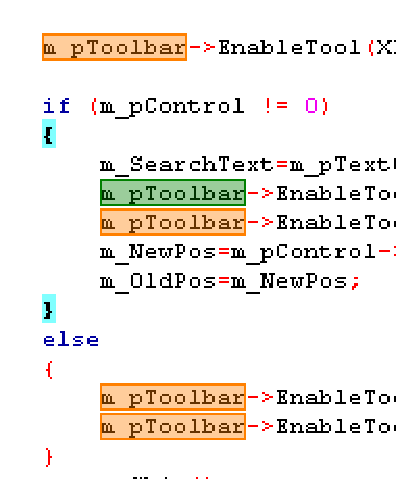
\includegraphics{incremental_search_example}

If the search term cannot be found within the active file, this fact is highlighted by the background of the search mask being displayed in red.

\begin{description}
\item[ESC] Leave the Incremental Search modus.
\item[ALT-DELETE] Clear the input of the incremental search field.
\end{description}

The icons in the Incremental Search toolbar have the following meanings:

\begin{description}
\item[
\includegraphics{incremental_search_clear}] Deleting the text within the search mask of the Incremental Search toolbar.
\item[
\includegraphics{incremental_search_previous},
\includegraphics{incremental_search_next}] Navigating between the occurrences of a search term.
\item[
\includegraphics{incremental_search_highlight}] Clicking this button results in all the occurrences of the search term within the editor being highlighted in colour, instead of only the initial occurrence.
\item[
\includegraphics{incremental_search_selected}] Activating this option restricts the search to the text passage marked within the editor.
\item[
\includegraphics{incremental_search_matchcase}] This option means a case sensitive search is performed.
\end{description}

\hint{The standard settings of this toolbar can be configured in \menu{Settings,Editor,Incremental Search}.}

\screenshot{incremental_search_settings}{Settings for Incremental Search}

\end{INCREMENTALSEARCH}

\begin{NASSISHNEIDERMAN}
\section{NassiShneiderman plugin}\label{sec:nassishneiderman}

NassiShneiderman plugin allows the creation of Nassi Shneiderman diagrams within \codeblocks (\cite{url:nassi}). 

\subsection{Create a diagram}

There are two possibilities to create a diagram.

\begin{enumerate}
\item To create an empty diagram select the menu options \menu{File,New,Nassi Shneiderman diagram}.
\item The second option is to creates a diagram from C/C++ source code. 
\end{enumerate}

In an editor window highlight some code to create the diagram from. For example the body of a function/method from the opening braces till the closing brace. Then right click the selection and choose \menu{Nassi Shneiderman,Create diagram} (see \pxref{fig:NassiShneidermanCreate1}). 

\screenshot{NassiShneidermanCreate1}{NassiShneiderman Create}

You should get a new diagram (see \pxref{fig:NassiShneidermanCreate2}).

\screenshot{NassiShneidermanCreate2}{NassiShneiderman Diagram Example}

The parser has some limitations:

\begin{itemize}
\item Comments can not be at the end of a branch.
\item From a definition of a function it is only able to parse the body, not the declaration.
\item For sure, you will find a lot more... 
\end{itemize}

\subsection{Editing structograms}
\subsubsection{What to do with a diagram?}

You can do a lot of things with a structogram:

\begin{enumerate}
\item Store for later usage. The diagram can be stored \menu{File,Save file} or \menu{File,Save file as...}.
\item It is possible to export to different formats \menu{File,Export}
    \begin{itemize}
    \item "Export source..." to save as C source file.
    \item "StrukTeX" to use in your documentation in LaTeX.
    \item "PNG" or "PS" and eventually "SVG" to have a diagram in an image format known by a lot of other tools.
    \end{itemize}        
\item Directly insert the code into the editor: Open or create a diagram. Back in an editor window right click and choose \menu{Nassi Shneiderman,insert from xy} (You get a list with all open diagrams here).
\item Drag'n'Drop the diagram (or parts of it) to other tools. For example to OpenOffice Writer to get an image in your documentation.
\end{enumerate}

If the chosen diagram has a selection, the export or code-generation takes only this part of the diagram. 

\subsubsection{Extensions}

The NassiShneiderman plugin supports some extensions of Nassi-Shneiderman diagrams: 

\begin{itemize}
\item break has a special brick with an "right-arrow"
\item continue has a special brick with a "left-arrow"
\item To be able to create diagrams from c/c++ switch statements, the selection does not implicitly break before a case. The different cases are vertically aligned. Supports C and C++.
\end{itemize}


\end{NASSISHNEIDERMAN}

\begin{LIBFINDER}
\section{LibFinder}\label{sec:lib_finder}

If you want to use some libraries in your application, you have to configure your project to use them. Such configuration process may be hard and annoying because each library can use custom options scheme. Another problem is that configuration differs on platforms which result in incompatibility between unix and windows projects.

LibFinder provides two major functionalities:

\begin{itemize}
\item Searching for libraries installed on your system
\item Including library in your project with just few mouse clicks making project platform-independent
\end{itemize}

\subsection{Searching for libraries}

Searching for libraries is available under \menu{Plugins,Library finder} menu. It's purpose is to detect libraries installed on your system and store the results inside LibFinder's database (note that these results are not written into \codeblocks project files). Searching starts with dialogue where you can provide set of directories with installed libraries. LibFinder will scan them recursively so if you're not sure you may select some generic directories. You may even enter whole disks -- in such case searching process will take more time but it may detect more libraries (see \pxref{fig:list_of_directories}).

\screenshot{list_of_directories}{List of directories}

When LibFinder scans for libraries, it uses special rules to detect presence of library. Each set of rules is located in xml file. Currently LibFinder can search for wxWidgets 2.6/2.8, \codeblocks SDK and GLFW -- the list will be extended in future.

\hint{To get more details on how to add library support into LibFinder, read \file{src/plugins/contrib/lib\_finder/lib\_finder/readme.txt} in \codeblocks sources.}

After completing the scan, LibFinder shows the results (see \pxref{fig:search_results}).

\screenshot{search_results}{Search results}

In the list you check libraries which should be stored into LibFinder's database. Note that each library may have more than one valid configuration and settings added ealier are more likely to be used while building projects.

Below the list you can select what to do with results of previous scans:

\begin{description}
\item[Do not clear previous results] This option works like an update to existing results -- it adds new ones and updates those which already exist. This option is not recommended.
\item[Second option (Clear previous results for selected libraries)] will clear all results for libraries which are selected before adding new results. This is the recommended option.
\item[Clear all previous library settings] when you select this option, LibFinder's database will be cleared before adding new results. It's useful when you want to clean some invalid LibFinder's database.
\end{description}

Another option in this dialogue is \menu{Set up Global Variables}. When you check this option, LibFinder will try automatically configure Global Variables which are also used to help dealing with libraries.

If you have pkg-config installed on your system (it's installed automatically on most linux versions) LibFinder will also provide libraries from this tool. There is no need to perform scanning for them -- they are automatically loaded when \codeblocks starts.

\subsection{Including libraries in projects}

LibFinder adds extra tab in Project Properties \menu{Libraries} -- this tab shows libs used in project and libs known in LibFinder. To add library into your project, select it in right pane and click $<$ button. To remove library from project, select it on the left pane and click $>$ button (see \pxref{fig:project_configuration}).

\screenshot{project_configuration}{Project configuration}

You can filter libraries known to LibFinder by providing search filter. The \menu{Show as Tree} checkbox allows to switch between categorized and uncategorized view.

If you want to add library which is not available in LibFinder's database, you may use \menu{Unknown Library} field. Note that you should enter library's shortcode (which usually matches global variable name) or name of library in pkg-config. List of suggested shortcodes can be found at \href{http://wiki.codeblocks.org/index.php?title=Recommended_global_variables}{Global Variables}. Using this option is recommended only when preparing project to be built on other machines where such library exists and is properly detected by LibFinder. You can access a global variable within \codeblocks like:

\begin{code}
$(#GLOBAL_VAR_NAME.include)
\end{code}

Checking the \menu{Don't setup automatically} option will notify LibFinder that it should not add libraries automatically while compiling this project. In such case, LibFinder can be invoked from build script. Example of such script is generated and added to project by pressing \menu{Add manual build script}.

\subsection{Using LibFinder and projects generated from wizards}

Wizards will create projects that don't use LibFinder. To integrate them with this plugin, you will have to manually update project build options. This can be easily achieved by removing all library-specific settings and adding library through \menu{Libraries} tab in project properties.

Such project becomes cross-platform. As long as used libs are defined in LibFinder's database, project's build options will be automatically updated to match platform-specific library settings.



\end{LIBFINDER}

\begin{SPELLCHECKER}
\section{SpellChecker plugin}\label{sec:spell_checker}

A plugin to check the spelling of strings and comments.

\subsection{Introduction}
A plugin to check the spelling of strings and comments. The spelling gets checked during typing. Additionally a thesaurus is provided. Both may be accessed on-demand by selecting the word in question, then choosing either Spelling... or Thesaurus... from the Edit menu (the operation can be bound to a hot-key via the Keyboard Shortcuts plugin). The context menu (right click the word) provides spelling suggestions. 

\subsection{Configuration}

Configuration is in the menu \menu{Settings,Editor}. The spell check option are about half way down the list on the left.

\screenshot{ConfigureSpellChecker}{SpellChecker Configuration}

The meaning of the controls are: 
\begin{description}
\item[Enable online spell checker] Enable or disable the spell checker.
\item[Language] The language used for spell checking and the thesaurus is selected by choosing a dictionary. This can also be changed in the status bar.
\item[Path settings, Dictionaries] The plugin is looking in this path for the dictionary files.
\item[Path settings, Thesauri] The plugin is looking in this path for the files needed by the thesaurus.
\item[Path settings, Bitmaps] (Optional) The plugin is looking in this path for the flags to show in the status bar.
\end{description}

\hint{You can use Macros in the above three path settings, such as \$(CODEBLOCKS)/share/codeblocks/SpellChecker. See Variable expansion for more details. This is quite convenient if you use portable \codeblocks.}

\subsection{Dictionaries}

SpellChecker uses a library called hunspell. Hunspell is the spell checker of OpenOffice.org, Mozilla Firefox and other projects. Dictionaries available for those applications are compatible with this plugin.

Open Office provides a collection of dictionaries for several languages and dialects to download. The OOo 3.x extensions (*.oxt) are compressed archives which can be opened with your favourite archiver (for example 7-Zip or File Roller). Copy the .aff file and the .dic file to the directory configured in 'Path settings, Dictionaries' (see above).

If you're running Linux you've probably already got compatible dictionaries installed. Look in /usr/share/hunspell or my choice is /usr/share/myspell/dicts. The reason I like the myspell files is they already include thesaurus files which are named correctly to work with the thesaurus, and everything is all in one location. Don't copy these files. Just point the spell checker to where the files are already located.

I understand on Windows, Firefox and Thunderbird also install compatible dictionary files. These can be found in... \file{C:\osp Program Files\osp Mozilla Firefox\osp dictionaries} or \file{C:\osp Program Files\osp Mozilla Thunderbird\osp dictionaries}. In addition, both OpenOffice.org and LibreOffice install dictionary files to\\ \file{C:\osp Program Files\osp (Open/Libre)Office\osp share\osp extensions\osp dict-*}.

The Google Chrome browser also installs dictionaries, but they are .bdic format and the \codeblocks spell checker plugin will not work with them.

\subsection{Thesaurus files}

The files for the thesaurus are also available from OOo, like the dictionaries. Copy the thesaurus files (th\_*.dat and th\_*.idx) to the directory configured in 'Path settings, Thesauri' (see above) and rename them to match the name of the dictionary but prepend "th\_" and let the extension as is.

\textbf{Example}: If the dictionary files (for one language) are "en\_GB.aff" and "en\_GB.dic" the files used for the thesaurus are "th\_en\_GB.idx" and "th\_en\_GB.dat".

On my Linux system I found thesaurus files already installed in /usr/share/myspell/dicts and /usr/share/mythes. Again, don't move the files. Set the spell checker to use the files from their current location.

On Windows, if either OpenOffice.org or LibreOffice is installed, they often include thesaurus files in \file{C:\osp Program Files\osp (Open/Libre)Office\osp share\osp extensions\osp dict-*}. 

\subsection{Bitmaps (flags)}

The bitmap of the actually selected language is shown in the status bar. If no bitmap is found, the name of the language is shown. The bitmap must be a PNG image. Choose a flag from the famfamfam\_flag\_icons and copy it to the directory configured in 'Path settings, Bitmaps' (see above) and rename it to match the name of the dictionary but let the extension png.

\subsection{Styles to check}

Only text with specific styles gets checked (for example only comments and strings). Styles are automatically set by Scintilla (CodeBlocks editing component).

The file OnlineSpellChecking.xml contains a list with indices of the styles to check. The indices differ for different programming-languages so the file contains a list for every programming-language. To add styles, look for the name of the programming-language and the indices in the corresponding lexer\_*.xml file and add this information to the file OnlineSpellChecking.xml.

For example, to check the spelling in bash shell scripts (*.sh files), add the line: 

\codeline{<Language name="Bash" index="2,5,6" />}
\end{SPELLCHECKER}

\begin{SRCEXPORTER}
\section{Source Code Exporter}\label{sec:src_exporter}

The necessity occurs frequently of transferring source code to other applications or to e-mails. If the text is simply copied, formatting will be lost, thus rendering the text very unclear.
The \codeblocks export function serves as a remedy for such situations. The required format for the export file can be selected via \menu{File,Export}. The program will then adopt the file name and target directory from the opened source file and propose these for saving the export file. The appropriate file extension in each case will be determined by the export format. The following formats are available.

\begin{description}
\item[html] A text-based format which can be displayed in a web browser or in word processing applications.
\item[rtf] The Rich Text format is a text-based format which can be opened in word processing applications such as Word or OpenOffice.
\item[odt] Open Document Text format is a standardised format which was specified by Sun and O'Reilly. This format can be processed by Word, OpenOffice and other word processing applications.
\item[pdf] The Portable Document Format can be opened by applications such as the Acrobat Reader.
\end{description}

\end{SRCEXPORTER}

\begin{SVN}
\section{SVN Support}\label{sec:svn}

The support of the version control system SVN is included in the \codeblocks plugin TortoiseSVN. Via the menu \menu{TortoiseSVN,Plugin settings} you can configure the accessible svn commands in the tab \menu{Integration}.

\begin{description}
\item[Menu integration] Add an entry TortoiseSVN with different settings in the menu bar.
\item[Project manger] Activate the TortoiseSVN commands in the context menu of the project manager.
\item[Editor] Active the TortoiseSVN commands in the context menu of the editor.
\end{description}

In the plugin settings you can configure which svn commands are accessible via the menu or the context menu. The tab integration provides the entry \menu{Edit main menu} and \menu{Edit popup menu} to configure these commands.

\hint{The File Explorer in \codeblocks uses different icon overlays for indicating the svn status. The TortoiseSVN commands are included here in the context menu.}

\end{SVN}

\begin{TODOLIST}
\section{ToDo List}\label{sec:todo_list}

In complex software projects, where different users are involved, there is often the requirement of different tasks to be performed by different users. For this purpose, \codeblocks offers a Todo List. This list can be opened via \menu{View,To-Do list}, and contains the tasks to be performed, together with their priorities, types and the responsible users. The list can be filtered for tasks, users and/or source files.

\screenshot{todo_list}{Displaying the ToDo List}

\hint{The To-Do list can be docked in the message console. Select the option \samp{Include the To-Do list in the message pane} via the menu \menu{Settings,Environment}.}

If the sources are opened in \codeblocks, a Todo can be added to the list via the context menu command \samp{Add To-Do item}. A comment will be added in the selected line of the source code.

\begin{code}
// TODO (user#1#): add new dialog for next release
\end{code}

When adding a To-Do, a dialogue box will appear where the following settings can be made (see \pxref{fig:add_todo}).

\figures[hbt!][width=.5\columnwidth]{add_todo}{Dialogue for adding a ToDo}

\begin{description}
\item[User] User name \var{user} in the operating system. Tasks for other users can also be created here. In doing so, the corresponding user name has to be created by Add new. The assignment of a Todo is then made via the selection of entries listed for the User.

\hint{Note that the Users have nothing to do with the Personalities used in \codeblocks.}
\item[Type] By default, type is set to Todo.
\item[Priority] The importance of tasks can be expressed by priorities (1 - 9) in \codeblocks.
\item[Position] This setting specifies whether the comment is to be included before, after or at the exact position of the cursor.
\item[Comment Style] A selection of formats for comments (e.g. doxygen).
\end{description}

\end{TODOLIST}

\begin{TOOLSPLUS}
\section{Tools+}\label{sec:tools+}

Creating a new tool is fairly simple, and can be completed in a few simple steps. First open \menu{Tools(+),Configure Tools...} to access the User-defined Tools dialog.

\figures{tools_setup}{User-defined Tools dialog}

\genterm{Tool Name}

This is the name that will be displayed in the Tools(+) drop-down menu. It will also be displayed as the tab name for tools that redirect to the Tools output window.

\genterm{Command Line}

Any valid command line function and switches can be placed here. Variable substitution is also accepted. The following list contains the more useful variables (see \pxref{sec:builtin_variables} for the full list).

\begin{codeentry}
\item[\$relfile, \$file] Respectively, the relative and absolute name of a selected file.
\item[\$reldir, \$dir] Respectively, the relative and absolute name of a selected directory.
\item[\$relpath, \$path] The relative and absolute name of the selected file or directory.
\item[\$mpaths] A list of selected files or directories (absolute paths only).
\item[\$fname, \$fext] The name without extension and the extension without the name of the selected file.
\item[\$inputstr\{prompt\}] Prompts the user to enter a string of text which is substituted into the command line.
\item[\$if(condition)\{true clause\}\{false clause\}] Resolves to \codeline{false clause} if \codeline{condition} is empty, 0, or false; otherwise \codeline{true clause}.
\end{codeentry}

\genterm{File Types}

Wildcard expressions separated by semicolons will restrict population of the right click menu of a file, directory, or multiple paths in the Project Tree, File Explorer, or Editor Pane to the specified type(s). Leave blank to handle all file/directory types.

\genterm{Working Directory}

The directory from which the command is executed. \codeblocks variables, project variables, and global variables are available. Also,

\begin{enumerate}
\item If \codeline{\$dir} is specified in the command line then \codeline{\$dir} may be used here as well.
\item \codeline{\$parentdir} is available for \codeline{\$relfile}, \codeline{\$file}, \codeline{\$reldir}, \codeline{\$dir}, \codeline{\$relpath}, \codeline{\$path}, \codeline{\$fname}, \codeline{\$fext}, evaluating into the absolute path of the directory containing the item.
\end{enumerate}

\genterm{Tools Menu Path}

Controls the placement of the command in the Tools(+) menu, giving the option of adding sub-menus (multiple levels are allowed).

\begin{itemize}
  \item Submenu/Tool1
  \item Submenu/Tool2
  \item Tool3
\end{itemize}

Will create this structure.

\figures{tools_menu_path}{Tools menu structure}

The command name will be used if this entry is blank. If the first character is a period, the command will be hidden.

\genterm{Context Menu Path}

This controls the command's placement in the right-click menu of the Projects and Files tabs of the Management pane. The same rules of structure with the Tools Menu Path apply here.

\figures{tools_context_path}{Context menu structure}

Please note that the command will not show up in the context menu unless the Command Line contains one or more of the following: \codeline{\$relfile}, \codeline{\$file}, \codeline{\$reldir}, \codeline{\$dir}, \codeline{\$relpath}, \codeline{\$path}, \codeline{\$fname}, and \codeline{\$fext}.

\genterm{Output to}

This determines where the output of the command will be redirected. The purpose and function of the command will determine which is best to select.
\genterm{Tools Output Window}
Tools that only output results command (and require no input) line generally use this setting. The program will be run invisibly and any output will be redirected to the appropriate tab of the Tools Output Window. The text [DONE] will be added upon the tool's completion.

\figures{tool_output}{Tool Output window}

\hint{If the Tools Output window is open when Code::Blocks is closed, it may trigger Code::Blocks to crash.}

\genterm{Code::Blocks Console}
This will cause the program to be run through the executable \file{cb\_console\_runner} (the same program that is launched after Build and run). This is generally used for command line tools with more advanced user interactions, although GUI programs can also be used (especially if the program is unstable and/or also leaves messages in the standard output). Console runner will pause the window (prevent it from closing), display the run time, and the exit code when the program finishes.
\genterm{Standard Shell}
This is the same as placing the command in a batch or shell script, then running it. The program will run in whatever its default method is, and when it finishes, its window will close. This setting is useful for running a program (for example a file or web browser) that must remain open after \codeblocks is closed.

\hint{As the Tools+ plugin is not yet complete, some functionality - specifically Menu Priority and Environment Variables - are not available.}

\subsection{Example Tools}

\genterm{Open file browser to selected file}

\begin{itemize}
\item Windows Explorer
\begin{itemize}
\item Tools Menu
\begin{cmd}
explorer /select,"$(PROJECTFILE)"
\end{cmd}
\item Context Menu
\begin{cmd}
explorer /select,"$path"
\end{cmd}
\end{itemize}

\item Dolphin
\begin{itemize}
\item Tools Menu
\begin{cmd}
dolphin --select "$(PROJECTFILE)"
\end{cmd}
\item Context Menu
\begin{cmd}
dolphin --select "$path"
\end{cmd}
\end{itemize}

\hint{The following three Context Menu commands only support folders (but not files).}

\item Nautilus
\begin{itemize}
\item Tools Menu
\begin{cmd}
nautilus --no-desktop --browser "$(PROJECTDIR)"
\end{cmd}
\item Context Menu
\begin{cmd}
nautilus --no-desktop --browser "$dir"
\end{cmd}
\end{itemize}

\item Thunar
\begin{itemize}
\item Tools Menu
\begin{cmd}
thunar "$(PROJECTDIR)"
\end{cmd}
\item Context Menu
\begin{cmd}
thunar "$dir"
\end{cmd}
\end{itemize}

\item PCMan File Manager
\begin{itemize}
\item Tools Menu
\begin{cmd}
pcmanfm "$(PROJECTDIR)"
\end{cmd}
\item Context Menu
\begin{cmd}
pcmanfm "$dir"
\end{cmd}
\end{itemize}
\end{itemize}

\genterm{Update Subversion directory}

\begin{itemize}
\item Windows
\begin{itemize}
\item Tools Menu
\begin{cmd}
"path_to_svn\bin\svn" update "$inputstr{Directory}"
\end{cmd}
\item Context Menu
\begin{cmd}
"path_to_svn\bin\svn" update "$dir"
\end{cmd}
\end{itemize}

\item Linux
\begin{itemize}
\item Tools Menu
\begin{cmd}
svn update "$inputstr{Directory}"
\end{cmd}
\item Context Menu
\begin{cmd}
svn update "$dir"
\end{cmd}
\end{itemize}
\end{itemize}

\genterm{Compress active project to archive}

\begin{itemize}
\item Windows
\begin{itemize}
\item 7z or zip - Tools Menu
\begin{cmd}
"path_to_7z\7z" a -t$if(zip == $inputstr{7z or zip?}){zip -mm=Deflate -mmt=on -mx9 -mfb=128 -mpass=10}{7z -m0=LZMA -mx9 -md=64m -mfb=64 -ms=on} -sccUTF-8 "-w$(PROJECTDIR).." "$(PROJECTDIR)..\$(PROJECT_NAME)" "$(PROJECTDIR)*"
\end{cmd}
\item tar.gz or tar.bz2 - Tools Menu
\begin{cmd}
cmd /c ""path_to_7z\7z" a -ttar -mx0 -sccUTF-8 "-w$(PROJECTDIR).." "$(PROJECTDIR)..\$(PROJECT_NAME)" "$(PROJECTDIR)*" && "path_to_7z\7z" a -t$if(gz == $inputstr{gz or bz2?}){gzip -mx9 -mfb=128 -mpass=10 -sccUTF-8 "-w$(PROJECTDIR).." "$(PROJECTDIR)..\$(PROJECT_NAME).tar.gz}{bzip2 -mmt=on -mx9 -md=900k -mpass=7 -sccUTF-8 "-w$(PROJECTDIR).." "$(PROJECTDIR)..\$(PROJECT_NAME).tar.bz2}" "$(PROJECTDIR)..\$(PROJECT_NAME).tar" && cmd /c del "$(PROJECTDIR)..\$(PROJECT_NAME).tar""
\end{cmd}

\hint{The Windows command line interpreter has been invoked directly here (\cmdline{cmd /c}), allowing for multiple commands to be chained in a single line. However, this causes the command to fail to execute in the Code::Blocks Console.}

\end{itemize}

\item Linux
\begin{itemize}
\item 7z or zip - Tools Menu
\begin{cmd}
7z a -t$if(zip == $inputstr{7z or zip?}){zip -mm=Deflate -mmt=on -mx9 -mfb=128 -mpass=10}{7z -m0=LZMA -mx9 -md=64m -mfb=64 -ms=on} -sccUTF-8 "-w$(PROJECTDIR).." "$(PROJECTDIR)../$(PROJECT_NAME)" "$(PROJECTDIR)*"
\end{cmd}
\item tar.gz or tar.bz2 - Tools Menu
\begin{cmd}
tar -cf "$(PROJECTDIR)../$(PROJECT_NAME).tar.$if(gz == $inputstr{gz or bz2?}){gz" -I 'gzip}{bz2" -I 'bzip2} -9' "$(PROJECTDIR)*"
\end{cmd}
\end{itemize}
\end{itemize}

\end{TOOLSPLUS}

\begin{THREADSEARCH}
\section{Thread Search}\label{sec:thread_search}

Via the \menu{Search,Thread Search} menu, the appropriate plug-in can be shown or hidden as a tab in the Messages Console. In \codeblocks, a preview can be displayed for the occurrence of a character string in a file, workspace or directory. In doing so, the list of search results will be displayed on the right-hand side of the ThreadSearch Console. By clicking an entry in the list, a preview is displayed on the left-hand side. By double-clicking in the list, the selected file is opened in the \codeblocks editor.

\hint{The scope of file extensions to be included in the search, is preset and might have to be adjusted.}

\subsection{Features}

ThreadSearch plugin offers the following features:

\begin{itemize}
\item Multi-threaded \samp{Search in files}
\item Internal read-only editor to preview the results
\item File open in editors notebook
\item Contextual menu \samp{Find occurrences} to start a search in files with the word under cursor
\end{itemize}

\screenshot[hbt!][width=\columnwidth]{threadsearch_panel}{Thread Search Panel}

\subsection{Usage}

\begin{enumerate}
\item Configure your search preferences (see \pxref{fig:threadsearch_options})

Once the plugin is installed, there are 4 ways to run a search:

\begin{enumerate}
\item Type/Select a word in the search combo box and press enter or click on Search on the Thread search panel of the Messages notebook.
\item Type/Select a word in the toolbar search combo box and press enter or click on Search button.
\item Right click on any \samp{word} in active editor and click on \samp{Find occurrences}.
\item Click on Search/Thread search to find the current word in active editor.
\hint{Items 1, 2 and 3 may not be available according to current configuration.}
\end{enumerate}
\item Click again on the search button to cancel current search.
\item A single click on a result item displays it on the preview editor at right location.
\item A double click on a result item opens or set an editor in editors notebook at right location.
\end{enumerate}

\subsection{Configuration}

To access ThreadSearch plugin configuration panel click on (see \pxref{fig:threadsearch_options}):

\screenshot{threadsearch_options}{Configuration of Thread Search}

\begin{enumerate}
\item Options button on Messages notebook Thread search panel.
\item Options button on Thread search toolbar.
\item Settings/Environment menu item and then on the Thread search item on the left columns.
\end{enumerate}

\hint{Items 1, 2 and 3 may not be available according to current configuration.}

Search in part defines the set of files that will be analysed.

\begin{itemize}
\item Project and Workspace checkboxes are mutually exclusive.
\item Directory path can be edited or set with Select button.
\item Mask is the set a file specifications separated by \samp{;}. For example: \file{*.cpp;*.c;*.h.}
\end{itemize}

\subsection{Options}

\begin{description}
\item[Whole word] if checked, line matches search expression if search expression is found with no alpha-numeric \codeline{+'_'} before and after.
\item[Start word] if checked, line matches search expression if search expression is found at the beginning of a word, ie no alpha-numeric \codeline{+'_'} before search expression.
\item[Match case] if checked, the search is case sensitive.
\item[Regular expression] the search expression is a regular expression.
\end{description}

\hint{If you want to search for regular expressions like \codeline{\n} you will have to set the option \menu{Use Advanced RegEx searches} via the menu \menu{Settings,Editor,General Settings}.}

\subsection{Thread search options}

\begin{description}
\item[Enable \samp{Find occurrences contextual menu item}] If checked, the Find occurrences of \samp{Focused word} entry is added to the editor contextual menu.
\item[Use default options when running \samp{Find occurrences}] If checked, a set of default options is applied to the searches launched with the \samp{Find occurrences} contextual menu item.Per defaut option \samp{Whole word} and \samp{Match case} is enabled.
\item[Delete previous results at search begin] If ThreadSearch is configured with \samp{Tree View} then the search results will be listet hierarchically,
\begin{itemize}
\item the first node contains the search term
\item above the files which contain the search term are listed
\item within this list the line number and the corresponding content of the occurence is displayed
\end{itemize}
If you search different terms the list will become confusing, therefore previous search results can be cleared at search begin using this option.
\hint{In the list of occurences single items or all items can be deleted via the context menu \menu{Delete item} or \menu{Delete all items}.}
\end{description}

\subsection{Layout}

\begin{description}
\item[Display header in log window] if checked, the header are displayed in the results list control.
\hint{If unchecked, the columns are no longer resizeable but space is spared.}
\item[Draw lines between columns] Draws lines between columns in list mode.
\item[Show ThreadSearch toolbar] Display the toolbar of Thread Search plugin.
\item[Show search widgets in ThreadSearch Messages panel] If checked, only the results list control and the preview editor are displayed. All other search widgets are hidden (spares space).
\item[Show code preview editor] Code preview can be hidden either with this check box or with a double click on the splitter window middle border. This is where it can be shown again.
\end{description}

\subsection{Panel Management}

You can choose different modes how the the ThreadSearch window is managed. With the setting \samp{Message Notebook} the ThreadSearch window will be a dockable window in the message panel. If you choose the setting \samp{Layout} you will be able to undock the window from the message panel and put it somewhere else.

\subsection{Logger Type}

The view of the search results can be displayed in different ways. The setting \samp{List} displays all occurrences as list. The other mode \samp{Tree} gathers all occurrences within a file as a node.

\subsection{Splitter Window Mode}

The user can configure a horizontal or vertical splitting of the preview window and the output window of the search results.

\subsection{Sort Search Results}

The view of the search results may be sorted by path or file name.

\end{THREADSEARCH}

\begin{MOREPLUGINS}
\section{Code statistics}

\screenshot{code_stats}{Konfiguration für Code Statistik}

Based on the entries in the configuration mask, this simple plugin detects the proportions of code, commentaries and blank lines for a project. The evaluation is called via the menu command \menu{Plugins,Code statistics}.

\section{Searching Available Source Code}

This plugin makes it possible to select a term within the editor and to search for this term via the context menu \menu{Search at Koders} in the \cite{url:koders} database. The dialogue offers the additional possibilities to of filtering for program languages and licences.

This database search will help you find source code originating from other world-wide projects of universities, consortiums and organisations such as Apache, Mozilla, Novell Forge, SourceForge and many others, which can be re-used without having to reinvent the wheel every time. Please observe the licence of the source code in each individual case.

\section{Code profiler}

A simple graphical interface to the GNU GProf Profiler.

\section{Symbol Table Plugin}

This plugin makes it possible to search for symbols in objects and libraries. The options and the path for the command line program nm are defined in the Options tab.

\screenshot{symtab_config}{Configuring the Symbol Table}

Clicking the \samp{Search} stats the search, the results of the NM program are displayed in a separate window caleld \samp{SymTabs Result}. The name of the objects or libraries containing the symbol are listed under the title \samp{NM's Output}.


\end{MOREPLUGINS}
